\begin{frame}[standout]
    Extra slides
\end{frame}



\begin{frame}{$\mathrm{NO_x}$ Emissions}

    $\mathrm{NO_x}$ emissions are a family of nitrogen oxides that are commonly associated with combustion processes of Ammonia.

    The key factors to reduce the $\mathrm{NO_x}$ emissions are combustion temperature and air-to-fuel ratio.

    \begin{figure}[H]
        \centering
        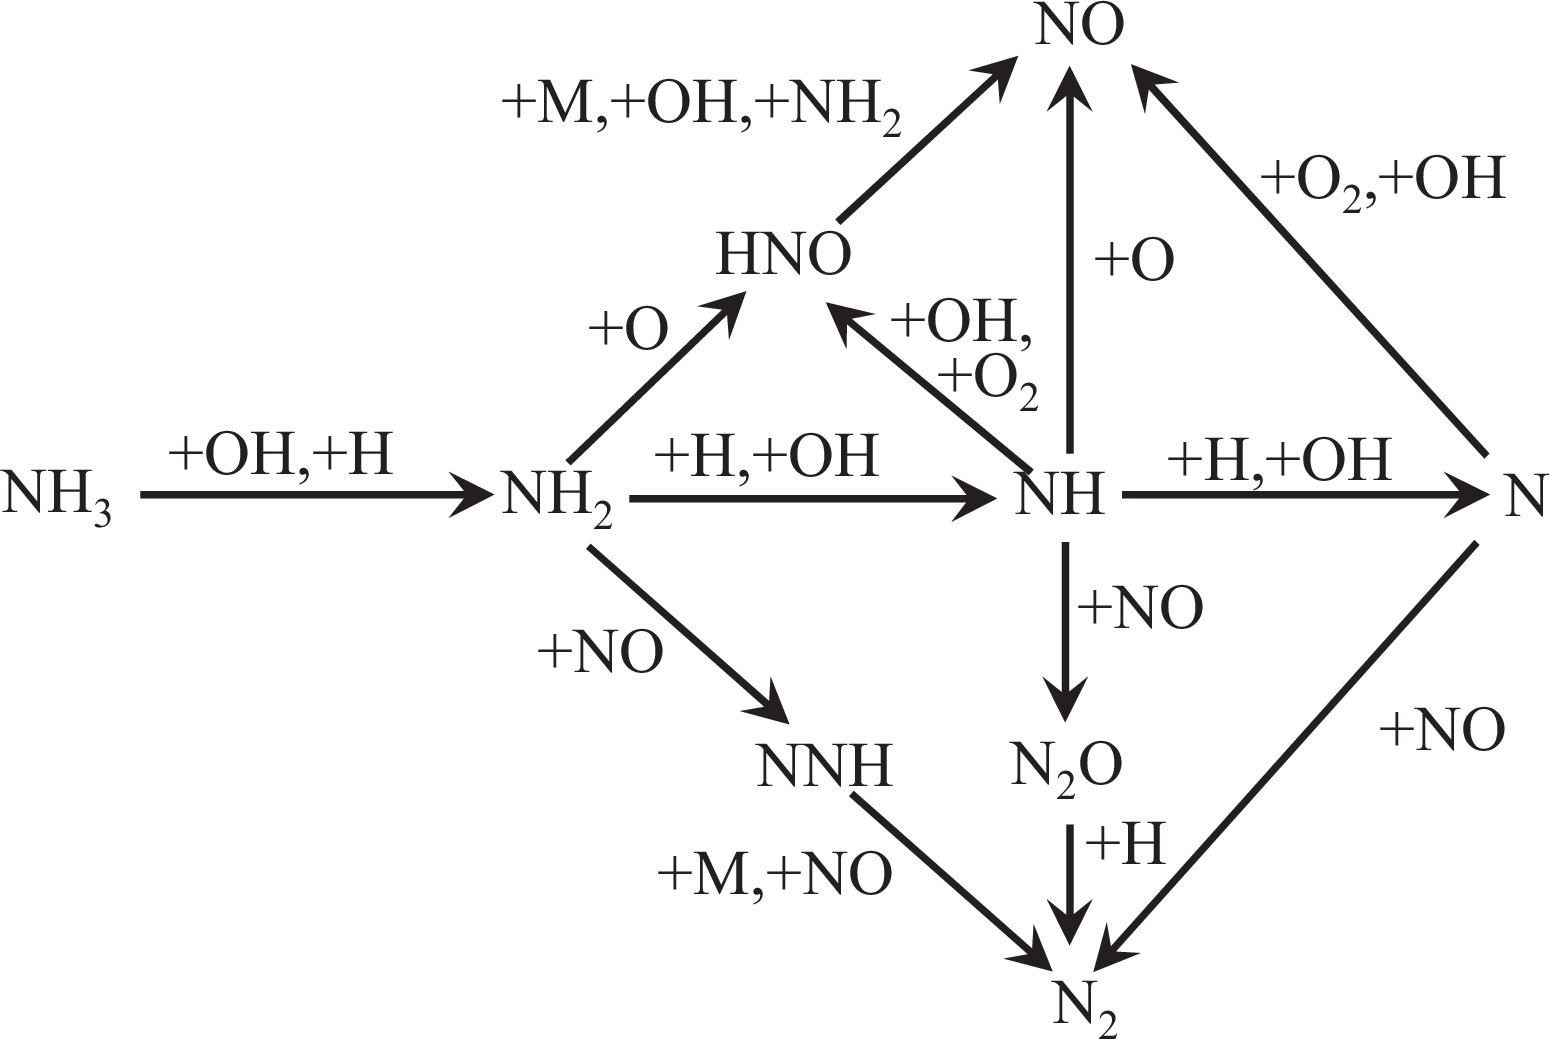
\includegraphics[width=0.6\textwidth]{img/NOx-emission-diagram.jpg}
        \caption{$\mathrm{NH_3}$ oxidation pathway.}
    \end{figure}

\end{frame}



\begin{frame}{Lagrangian vs. Eulerian CFD solver}

    \begin{columns}

        \begin{column}{0.5\textwidth}

            Lagrangian approach consists in \textbf{following droplets during their movement}.

            \begin{figure}[H]
                \centering
                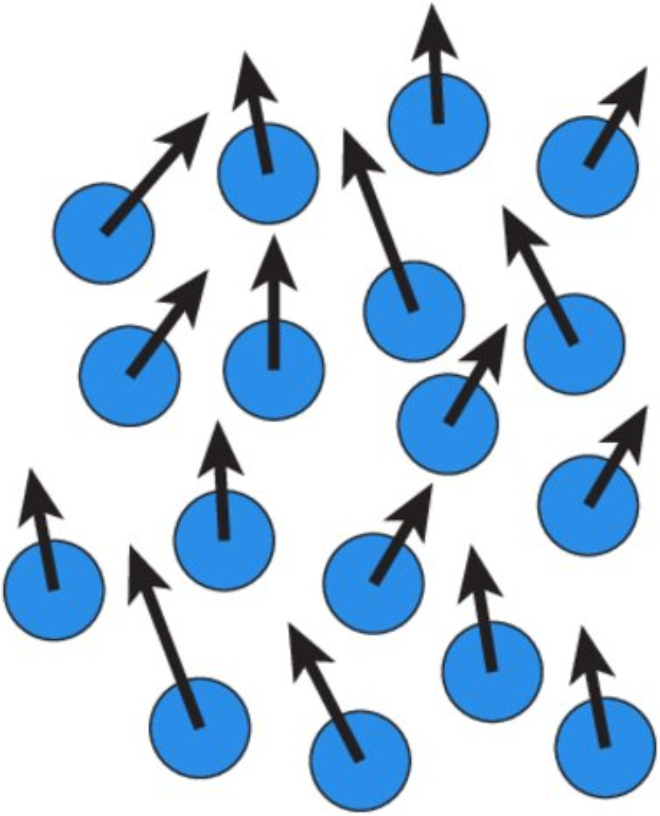
\includegraphics[height=0.5\textheight]{img/extra-lagrangian-approach.png}
                \caption{Lagrangian approach.}
            \end{figure}

        \end{column}

        \begin{column}{0.5\textwidth}

            Eulerian approach consists in \textbf{considering inlet and outlet flux in a given volume}.

            \begin{figure}[H]
                \centering
                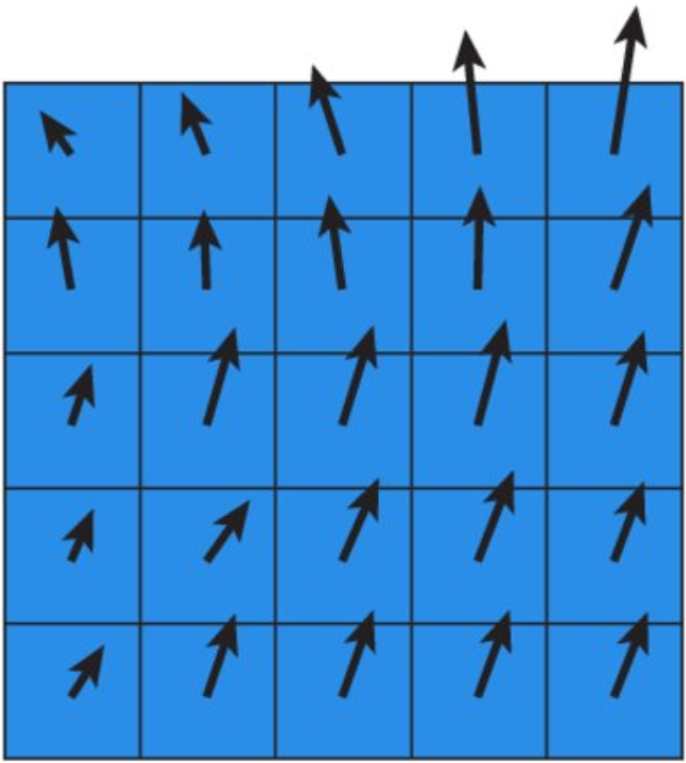
\includegraphics[height=0.5\textheight]{img/extra-eulerian-approach.png}
                \caption{Eulerian approach.}
            \end{figure}

        \end{column}

    \end{columns}

\end{frame}

% \begin{frame}
%     More of the different types of NOx emissions
%     More of the different types of fuel injectors
%     Who uses a suitable replacing combution chamber, what's our target?
% \end{frame}